\documentclass[10pt,a4paper]{report}
\usepackage[utf8]{inputenc}
\usepackage{amsmath}
\usepackage{mathtools}
\usepackage{amsfonts}
\usepackage{amssymb}
\usepackage{graphicx}
\usepackage{hyperref}
\usepackage{bm}
\usepackage{gensymb}
\usepackage{listings}
\usepackage[left=2cm,right=2cm,top=2cm,bottom=2cm]{geometry}
\usepackage{breqn}
\setlength\parindent{0pt}
\graphicspath{{./images/}}
\newcommand{\legendre}[2]{(\frac{#1}{#2})}

\begin{document}


\textbf{CATAM Part II - 14.6 - Isolating Integrals for Geodesic Motion}

\subsection*{Introduction}

Throughout this project I code in python, making use of the SymPy package for symbolic mathematics. The GraviPy package provides data structures to store and manipulate the kinds of tensors that appear in general relativity. We'll only need it to compute the Christoffel symbols. SciPy will be used to perform numerical integration. We use the +--- signature. 
\subsection*{Question 1}

We use the equivalent action 

\begin{equation*}
\mathcal{S}=\int \mathcal{L} d\tau
\end{equation*}
\begin{equation*}
\mathcal{L}=g_{ij}\dot{x}^i\dot{x}^j = g_{tt}\dot{t}^2 + 2g_{t\phi}\dot{t}\dot{\phi}+g_{\phi\phi}\dot{\phi}^2+g_{rr}\dot{r}^2+g_{\theta\theta}\dot{\theta}^2
\end{equation*} 

where the dot denotes differentiation with respect to $\tau$. This is valid since $\tau$ is an affine parameter, so gives the same geodesic equation as the Lagrangian with a square root. The conserved quantities come from the lack of dependence of $\mathcal{L}$ on $t, \phi$.\\

No $t$ dependence gives

\begin{equation}
\frac{\partial \mathcal{L}}{\partial \dot{t}} = 2g_{tt}\dot{t} + 2g_{t\phi}\dot{\phi} = 2E
\end{equation}

for $E$ constant, and similarly no $\phi$ dependence gives 

\begin{equation}
\frac{\partial \mathcal{L}}{\partial \dot{\phi}} = 2g_{t\phi}\dot{t}+2g_{\phi\phi}\dot{\phi} = -2L_z
\end{equation}

for $L_z$ constant. Rewriting these for later use we have: 

\begin{equation}
E = g_{tt}\dot{t} + g_{t\phi}\dot{\phi}
\label{Edef}
\end{equation}

\begin{equation}
L_z = - ( g_{t\phi}\dot{t}+g_{\phi\phi}\dot{\phi})
\label{Ldef}
\end{equation}

We get a further conserved quantity from no $\tau$ dependence

\begin{equation}
\mathcal{L} - \dot{x}^i \frac{\partial \mathcal{L}}{\partial \dot{x}^i} = -\mathcal{L} = -1
\label{Qdef}
\end{equation}

where $\mathcal{L} = 1$ is by timelikeness \footnote{with the +--- signature} \\

(\ref{Edef}) and (\ref{Ldef}) give a system of 2 equations for $\dot{t}, \dot{\phi}$ which can be solved to give

\begin{equation}
\dot{t} = \frac{Eg_{\phi\phi}+L_zg_{t\phi}}{g_{tt}g_{\phi\phi}-g_{t\phi}^2}
\label{tdef}
\end{equation}

\begin{equation}
\dot{\phi} = -\frac{Eg_{t\phi}+L_zg_{tt}}{g_{tt}g_{\phi\phi}-g_{t\phi}^2}
\label{phidef}
\end{equation}

which can be substituted into $\mathcal{L}=1$  to give (after some simple but tedious algebra): 

\begin{equation}
g_{rr}\dot{r}^2+g_{\theta\theta}\dot{\theta}^2 = -V_{eff}(r, \theta, E, L_z)
\label{effpot}
\end{equation}
\begin{equation*}
V_{eff}(r, \theta, E, L_z) = -1 + \frac{E^2g_{\phi\phi} + L_z^2g_{tt} + 2ELg_{t\phi}}{g_{tt}g_{\phi\phi}-g_{t\phi}^2}
\end{equation*}

\subsection*{Question 2}
Computing the Christoffel symbols and returning latex is pretty straightforward using GraviPy, and was done using $compute\_kerr\_christoffel.py$. We make some attempt to simplify the expressions through substitutions of $\Sigma$ and $\Delta$ post computation, however our program certainly misses some simplifcations. This won't matter for numerical calculation later. Displaying up to symmetry in the lower indices we get: \\



\small\begin{align*}
\Gamma^t_{tr} = - \frac{m \left(a^{2} + r^{2}\right) \left(a^{2} \cos^{2}{\left(\theta \right)} - r^{2}\right)}{\Delta \Sigma^{2}}\\
\Gamma^t_{t\theta} = - \frac{a^{2} m r \sin{\left(2 \theta \right)}}{\Sigma^{2}}\\
\Gamma^t_{r\phi} = - \frac{a m \left(2 \Sigma r^{2} + a^{4} \sin^{2}{\left(\theta \right)} - a^{4} + a^{2} r^{2} \sin^{2}{\left(\theta \right)} + r^{4}\right) \sin^{2}{\left(\theta \right)}}{\Delta \Sigma^{2}}\\
\Gamma^t_{\theta\phi} = \frac{a m r \left(- \Delta \Sigma + a^{4} - 2 a^{2} m r + 2 a^{2} r^{2} - 2 m r^{3} + r^{4}\right) \sin{\left(2 \theta \right)}}{\Delta \Sigma^{2}}\\
\Gamma^r_{tt} = \frac{\Delta m \left(- a^{2} \cos^{2}{\left(\theta \right)} + r^{2}\right)}{\Sigma^{3}}\\
\Gamma^r_{t\phi} = \frac{\Delta a m \left(a^{2} \cos^{2}{\left(\theta \right)} - r^{2}\right) \sin^{2}{\left(\theta \right)}}{\Sigma^{3}}\\
\Gamma^r_{rr} = \frac{r}{\Sigma} + \frac{m}{\Delta} - \frac{r}{\Delta}\\
\Gamma^r_{r\theta} = - \frac{a^{2} \sin{\left(2 \theta \right)}}{2 \Sigma}\\
\Gamma^r_{\theta\theta} = - \frac{\Delta r}{\Sigma}\\
\Gamma^r_{\phi\phi} = \frac{\Delta \left(- 8 \Sigma^{2} r + a^{4} m \left(\cos{\left(4 \theta \right)} - 1\right) + 8 a^{2} m r^{2} \sin^{2}{\left(\theta \right)}\right) \sin^{2}{\left(\theta \right)}}{8 \Sigma^{3}}\\
\Gamma^\theta_{tt} = - \frac{a^{2} m r \sin{\left(2 \theta \right)}}{\Sigma^{3}}\\
\Gamma^\theta_{t\phi} = \frac{a m r \left(a^{2} + r^{2}\right) \sin{\left(2 \theta \right)}}{\Sigma^{3}}\\
\Gamma^\theta_{rr} = \frac{a^{2} \sin{\left(2 \theta \right)}}{2 \Delta \Sigma}\\
\Gamma^\theta_{r\theta} = \frac{r}{\Sigma}\\
\Gamma^\theta_{\theta\theta} = - \frac{a^{2} \sin{\left(2 \theta \right)}}{2 \Sigma}\\
\Gamma^\theta_{\phi\phi} = - \frac{\left(\Sigma \left(\Delta \Sigma + 2 a^{2} m r + 2 m r^{3}\right) + 2 a^{2} m r \left(a^{2} + r^{2}\right) \sin^{2}{\left(\theta \right)}\right) \sin{\left(\theta \right)} \cos{\left(\theta \right)}}{\Sigma^{3}}\\
\Gamma^\phi_{tr} = \frac{a m \left(- a^{2} \cos^{2}{\left(\theta \right)} + r^{2}\right)}{\Delta \Sigma^{2}}\\
\Gamma^\phi_{t\theta} = - \frac{2 a m r}{\Sigma^{2} \tan{\left(\theta \right)}}\\
\Gamma^\phi_{r\phi} = \frac{\Sigma^{2} r - 2 \Sigma m r^{2} - \frac{a^{4} m \left(\cos{\left(4 \theta \right)} - 1\right)}{8} - a^{2} m r^{2} \sin^{2}{\left(\theta \right)}}{\Delta \Sigma^{2}}\\
\Gamma^\phi_{\theta\phi} = \frac{\Delta \Sigma^{2} - 2 \Delta \Sigma m r + 2 \Sigma a^{2} m r + 2 \Sigma m r^{3} + 2 a^{4} m r \sin^{2}{\left(\theta \right)} - 4 a^{2} m^{2} r^{2} + 2 a^{2} m r^{3} \sin^{2}{\left(\theta \right)} - 4 m^{2} r^{4}}{\Delta \Sigma^{2} \tan{\left(\theta \right)}}\\
\end{align*}

\normalsize

\subsection*{Programming Task}

The file $integrate.py$ contains all our integration code. It takes as inputs initial values of the 8 dynamic variables, as well as $\Gamma, m$ and $a$, defines the 4 geodesic equation ODEs and passes them to the $odeint$ function from SciPy. We'll need to come back and fiddle with some parameters later to ensure our integration gives us a smooth enough curve for our purposes. 
 
\subsection*{Question 3}

We could set $a=0$ in our Kerr Christoffel symbols, but find it much easier to calculate them from directly from the Schwartzchild metric. Using a section of $q3.py$:

\small\begin{align*}
\Gamma^t_{tr} = \frac{m}{r (- 2 m + r)}\\
\Gamma^r_{tt} = \frac{m (- 2 m + r)}{r^{3}}\\
\Gamma^r_{rr} = \frac{m}{r (2 m - r)}\\
\Gamma^r_{\theta\theta} = 2 m - r\\
\Gamma^r_{\phi\phi} = (2 m - r) \sin^{2}{(\theta )}\\
\Gamma^\theta_{r\theta} = \frac{1}{r}\\
\Gamma^\theta_{\phi\phi} = - \frac{\sin{(2 \theta )}}{2}\\
\Gamma^\phi_{r\phi} = \frac{1}{r}\\
\Gamma^\phi_{\theta\phi} = \frac{1}{\tan{(\theta )}}\\
\end{align*}

\normalsize
Now substituting $\theta=\pi/2$, $g_{\phi\phi} = -r^2$, $g_{tt}=(1-2m/r)$ and $g_{t\phi} = 0$ into (\ref{effpot}), we get:

\begin{equation}
V_{eff}(r, E, L_z) = -1 + \frac{E^2}{1-2m/r} - \frac{L^2}{r^2} = g_{rr}\dot{r}^2+g_{\theta\theta}\dot{\theta}^2
\label{SCVeff}
\end{equation}

which has zeros as solutions of 

\begin{equation*}
r^3(E^2-1) + 2mr^2 -L_z^2r+2mL_z^2=0
\end{equation*}

which for $E=0.97, L_z=4, m=1$ are $\approx 3.07, 7.61, 23.16$. By graphing, our potential is positive for $7.61<r<23.16$ or $2<r<3.07$, which are the allowed regions for bound orbits.

%Now a bound orbit in the equatorial plane must have $\dot{\theta}=0$, and so (\ref{SCVeff}) becomes

%\begin{equation*}
%\dot{r}^2 = -(1-2/r)V_{eff}
%\end{equation*}

%Only some of these solutions will be bound... TODO

\subsubsection*{3a}

Using (\ref{tdef}), (\ref{phidef}) and (\ref{SCVeff}) we can calculate initial values for $\dot{t}, \dot{\phi}$ and $\dot{\theta}$ respectively. Calling the function $compute\_one\_geodesic()$ in $q3.py$ does this computation of initial conditions, calls our integration function and then processes its output. \\

We produce the following plots using parameters $r=15, \theta=\pi/2, \dot{r}=0, E=0.97, L=4$. Some fiddling around with the integration parameters was required to get a smooth enough curve, and to find the correct $\tau$ range to give a few orbits. Looking at the $\phi$ plot, here we have just over 3 orbits. We calculate and plot $E$, $L_z$, and $g_{rr}\dot{r}^2+g_{\theta\theta}\dot{\theta}^2 + V_{eff}(r, \theta, E, L_z)$ at each point and see our 3 conservation laws to high precision, assuring us the numerical integration is accurate enough for our purposes.

\begin{figure}[!ht]
\begin{minipage}[b]{0.5\linewidth}
\centering
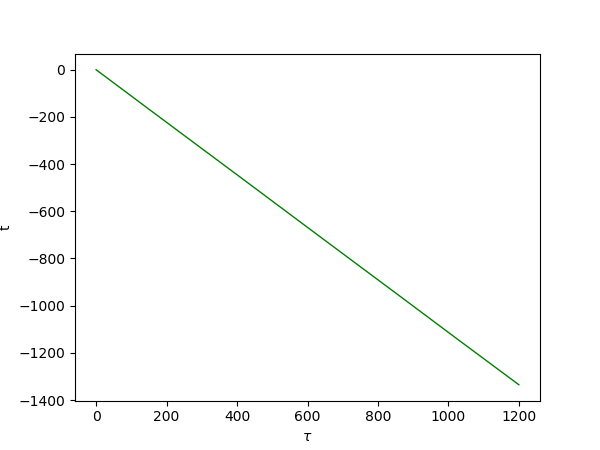
\includegraphics[width=\textwidth]{3a/t.png}
\caption{$t$}
\label{fig:figure1}
\end{minipage}
\hspace{0.5cm}
\begin{minipage}[b]{0.5\linewidth}
\centering
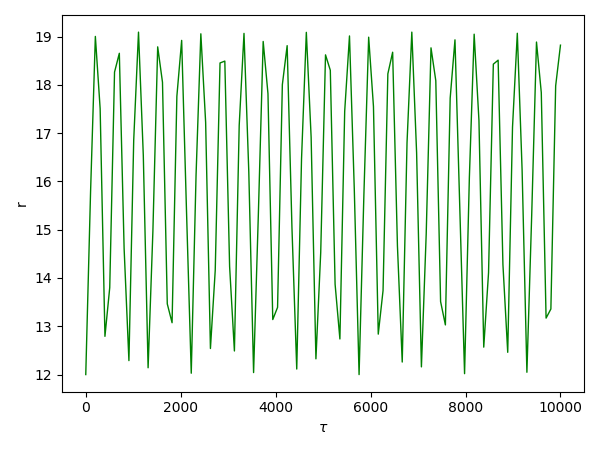
\includegraphics[width=\textwidth]{3a/r.png}
\caption{$r$}
\label{fig:figure2}
\end{minipage}
\end{figure}

\begin{figure}[!ht]
\begin{minipage}[b]{0.5\linewidth}
\centering
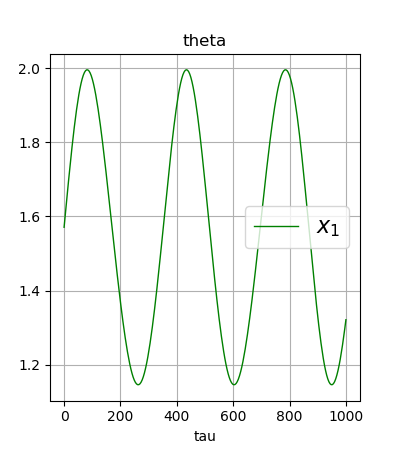
\includegraphics[width=\textwidth, height=6.5cm]{3a/theta.png}
\caption{$\theta$}
\label{fig:figure1}
\end{minipage}
\hspace{0.5cm}
\begin{minipage}[b]{0.5\linewidth}
\centering
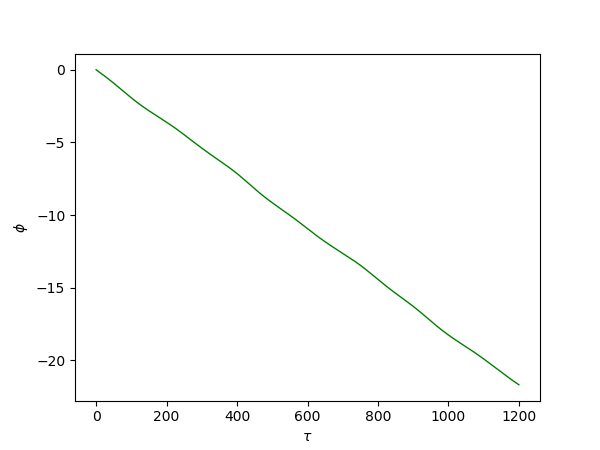
\includegraphics[width=\textwidth]{3a/phi.png}
\caption{$\phi$}
\label{fig:figure2}
\end{minipage}
\end{figure}

\begin{figure}[!ht]
\begin{minipage}[b]{0.5\linewidth}
\centering
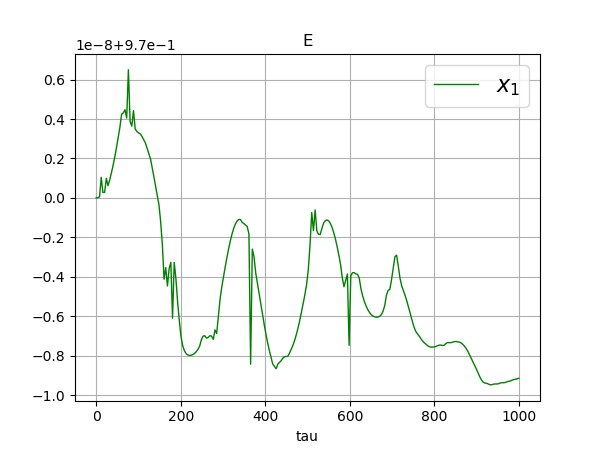
\includegraphics[width=\textwidth]{3a/E.png}
\caption{$E$}
\label{fig:figure1}
\end{minipage}
\hspace{0.5cm}
\begin{minipage}[b]{0.5\linewidth}
\centering
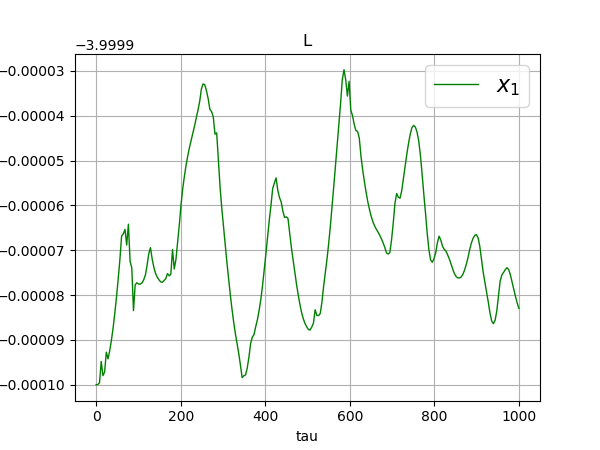
\includegraphics[width=\textwidth]{3a/L.png}
\caption{$L$}
\label{fig:figure2}
\end{minipage}
\end{figure}

\begin{figure}[!ht]
\begin{minipage}[b]{0.5\linewidth}
\centering
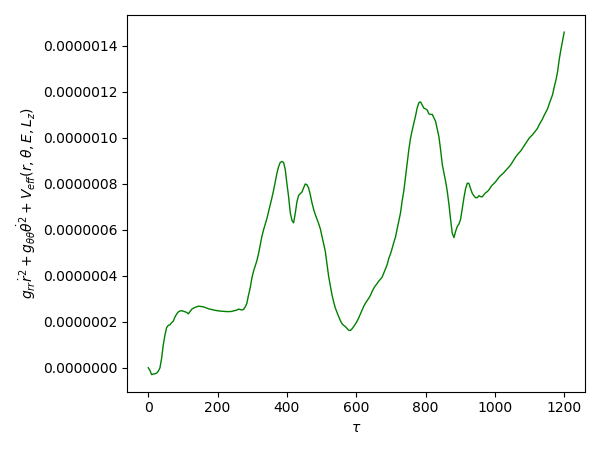
\includegraphics[width=\textwidth]{3a/Veff.png}
\caption{$g_{rr}\dot{r}^2+g_{\theta\theta}\dot{\theta}^2 + V_{eff}(r, \theta, E, L_z)$}
\label{fig:figure1}
\end{minipage}
\end{figure}

\newpage

\subsubsection*{3b}

We find as expected our code runs into issues if r is not in the range defined previously. Running the code listed under 3b in $q3.py$ with several $r_0$ values  we obtain for fixed $\theta=\pi/2, \dot{r_0}=0, E=0.97, L=4$ the following plots. We see the values form a closed curve under these conditions, with the shape of curve depending on the initial parameters

\begin{figure}[!ht]
\begin{minipage}[b]{0.5\linewidth}
\centering
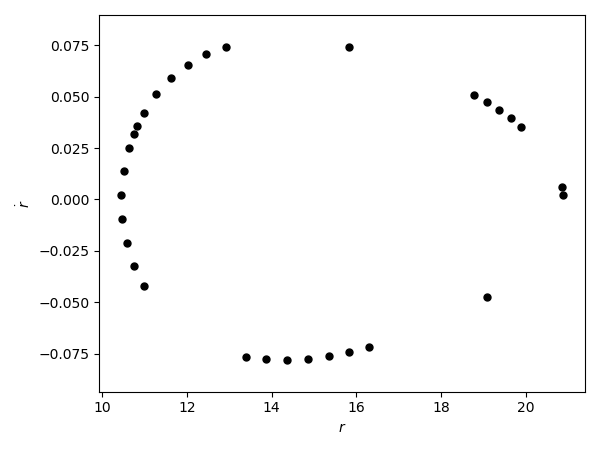
\includegraphics[width=\textwidth]{3b/r0=10,E=0.97,L=4.png}
\caption{$r_0=10$}
\label{fig:figure1}
\end{minipage}
\hspace{0.5cm}
\begin{minipage}[b]{0.5\linewidth}
\centering
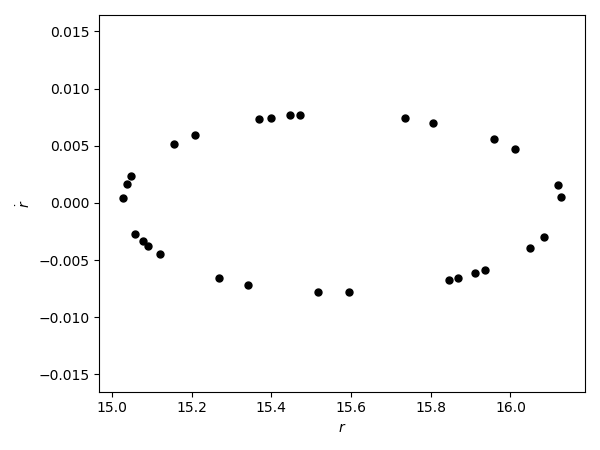
\includegraphics[width=\textwidth]{3b/r0=15,E=0.97,L=4.png}
\caption{$r_0=15$}
\label{fig:figure2}
\end{minipage}
\end{figure}

\begin{figure}[!ht]
\begin{minipage}[b]{0.5\linewidth}
\centering
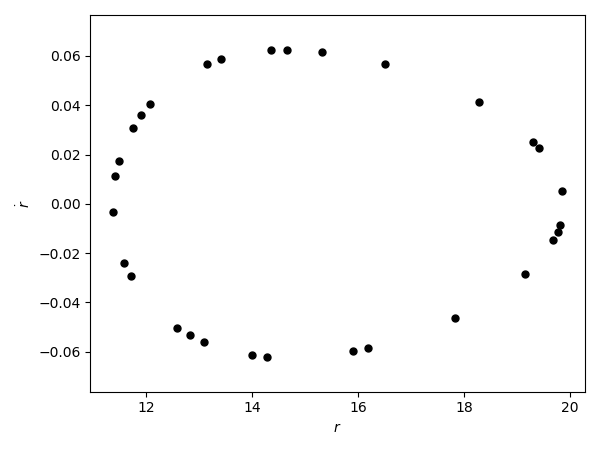
\includegraphics[width=\textwidth]{3b/r0=20,E=0.97,L=4.png}
\caption{$r_0=20$}
\label{fig:figure1}
\end{minipage}
\end{figure}



\newpage

\subsection*{Question 4}

Plotting the potential using $q4.py$ and using a numerical root finder, we see the allowed $r_0$ range with positive potential is $4.513<_0r<14.564$. Now modifying $q3.py$ to accommodate the Kerr metric, we produce the following Poincare maps, which all look very much like the Schwartzchild ones.

\begin{figure}[!ht]
\begin{minipage}[b]{0.5\linewidth}
\centering
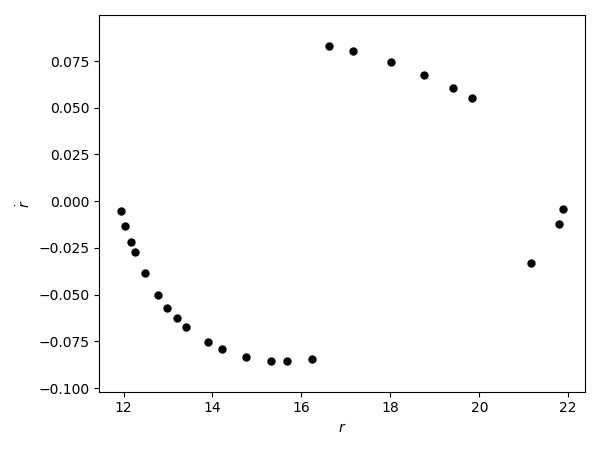
\includegraphics[width=\textwidth]{4/r0=8.png}
\caption{$r_0=10$}
\label{fig:figure1}
\end{minipage}
\hspace{0.5cm}
\begin{minipage}[b]{0.5\linewidth}
\centering
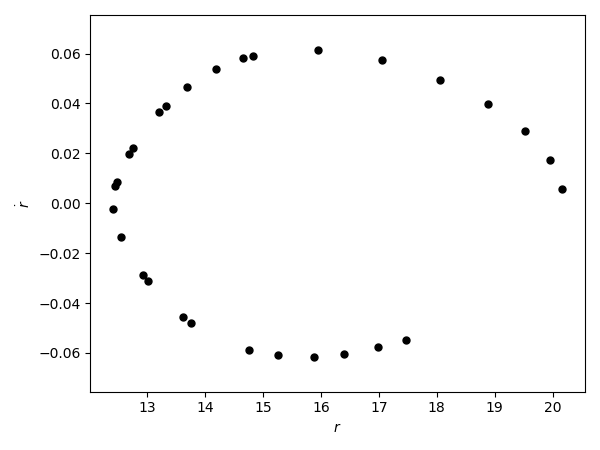
\includegraphics[width=\textwidth]{4/r0=10.png}
\caption{$r_0=15$}
\label{fig:figure2}
\end{minipage}
\end{figure}

\begin{figure}[!ht]
\begin{minipage}[b]{0.5\linewidth}
\centering
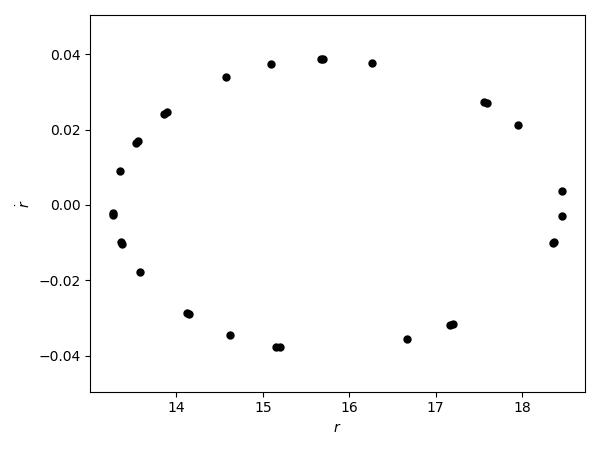
\includegraphics[width=\textwidth]{4/r0=12.png}
\caption{$r_0=20$}
\label{fig:figure1}
\end{minipage}
\end{figure}




\subsection*{Question 5}
The closedness of the Poincare plots suggests a quantity is preserved and we seek to show $Q$ is such. The script $q5.py$ attempts to symbolically simplify a hand computed expression for $\dot{Q}$. It first substitutes in an expression for $\ddot{\theta} = \ddot{\theta}(r,m,a,\theta,\dot{\theta}, \dot{t}, \dot{r},\dot{\phi})$ from the geodesic equation and Christoffel symbols. It then uses (\ref{Edef}), (\ref{Ldef}) and (\ref{Qdef}) to eliminate as many degrees of freedom as possible, and then we hope it simplifies sufficiently to let us read off $\delta$. I couldn't manage to get this to work, and my script kept giving horrendously complicated expressions that couldn't be simplified by eye.\\

In the $a=0$ limit Q becomes

\begin{equation*}
Q = L_z^2\csc^2{\theta} + r^2\dot{\theta}^2
\end{equation*}

choosing $\theta(\tau) = \pi/2$, which we are always free to do, we get 

\begin{equation*}
Q = L_z^2
\end{equation*}

the square of the total orbital angular momentum, which in this limit is dependent on our other constants $(L_z, E)$. In the general case general, this constant is known as the Carter constant\footnote{see for instance https://en.wikipedia.org/wiki/Carter_constant}, which is independent of $(L_z, E)$ and the three give enough conserved quantities to determine orbits uniquely given initial conditions. It doesn't seem immediately obvious what physical quantity it represents - a "hidden" symmetry if you will.


\newpage
\subsection*{Code}


\subsubsection*{compute\_kerr\_christoffel.py}
\small
\begin{verbatim}
from gravipy.tensorial import Coordinates, MetricTensor, All, Christoffel
from sympy import *
from gravipy import *

t, phi, r, theta, m, a, sigma, delta, sigma_for_printing, delta_for_printing = symbols('t, \phi, r, \\theta,
 m, a, sigma, delta, Sigma, Delta')
# chi is 4 vector of coords
x = Coordinates('\chi', [t, r, theta, phi])
sigma = r ** 2 + (a ** 2) * cos(theta) ** 2
delta = r ** 2 - 2 * m * r + a ** 2

Metric = Matrix([[(1 - (2 * m * r) / sigma), 0, 0, (2 * a * m * r * sin(theta) ** 2) / sigma], 
[0, -sigma / delta, 0, 0], [0, 0, - sigma, 0], 
[(2 * a * m * r * sin(theta) ** 2) / sigma, 0, 0,
 -(sin(theta) ** 2) * ((r ** 2 + a ** 2) + (2 * (a ** 2) * m * r * sin(theta) ** 2) / sigma)]])


g = MetricTensor('g', x, Metric)
Gamma = Christoffel('Gamma', g)

translate={1: "t", 2: "r", 3: "\\theta", 4: "\phi"}

for i in range(1,5):
    for j in range(1,5):
        for k in range(j,5):
            symbol = Gamma(-i,j,k)
            for l in range(1,5):
                symbol = symbol.subs(r ** 2 + (a ** 2) * cos(theta) ** 2, sigma_for_printing)
                symbol = symbol.subs(r ** 2 - 2 * m * r + a ** 2, delta_for_printing)
                symbol = symbol.subs(sigma_for_printing * a ** 2 + sigma_for_printing * r ** 2 
                - 2 * a ** 2 * m * r * cos(theta) ** 2 - 2 * m * r ** 3, sigma_for_printing * delta_for_printing )
                symbol=symbol.simplify()
            # to factorise product of delta and sigma
            symbol = symbol.subs(
                sigma_for_printing * a ** 2 + sigma_for_printing * r ** 2 + 2 * a ** 2 * m * r * sin(
                    theta) ** 2,
                sigma_for_printing * delta_for_printing + 2 * a ** 2 * m * r + 2 * m * r ** 3)
            symbol = symbol.simplify()

            for l in range(1, 5):
                symbol = symbol.subs(r ** 2 + (a ** 2) * cos(theta) ** 2, sigma_for_printing)
                symbol = symbol.subs(r ** 2 - 2 * m * r + a ** 2, delta_for_printing)
                symbol = symbol.subs(
                    sigma_for_printing * a ** 2 + sigma_for_printing * r ** 2 - 2 * a ** 2 * m * r * cos(
                        theta) ** 2 - 2 * m * r ** 3, sigma_for_printing * delta_for_printing)
                symbol = symbol.simplify()

            symbol = symbol.subs(
                sigma_for_printing * a ** 2 + sigma_for_printing * r ** 2 + 2 * a ** 2 * m * r * sin(
                    theta) ** 2,
                sigma_for_printing * delta_for_printing + 2 * a ** 2 * m * r + 2 * m * r ** 3)
            symbol = symbol.simplify()

            if symbol !=0:
                print("\Gamma^"+ translate[i]+"_{" + translate[j] + translate[k] + "} = " + 
                  latex(symbol) + r"\\")
\end{verbatim}
\normalsize
\subsubsection*{integrate.py}
\small
\begin{verbatim}
from collections import defaultdict
from scipy.integrate import odeint
from sympy import *
from numpy import loadtxt
from matplotlib.font_manager import FontProperties

def integrate(t,r,theta,phi,tdot,rdot,thetadot,phidot, m0, a0, Gamma):
    # initial values inputted, as well as christoffel symbols


    def vectorfield(w, tau, p):
        t, phi, r, theta, m, a= symbols('t, \phi, r, \\theta, m, a')
        """
        Defines the differential equations, and outputs an f

        Arguments:
            w :  vector of the state variables:
                      w = [x1,y1,x2,y2,x3,y3,x4,y4]
            tau :  time
            p :  vector of the parameters:
                      p = [m]
        """
        x1, y1, x2, y2, x3, y3, x4, y4 = w
        x=[x1,x2,x3,x4]
        y=[y1,y2,y3,y4]
        m0 = p[0]
        a0 = p[1]

        #compute DE for yi:
        ydot=defaultdict(float)
        for i in range(1,5):
            for j in range (1,5):
                for k in range (1,5):
                    ydot[i] += (-Gamma(-i,j,k)).subs([(t,x1),(r,x2),(theta,x3), (phi,x4), (m,m0), 
                    (a,a0)])*y[j-1]*y[k-1] #-1 as python list

        # Create f = (x1',y1',x2',y2'):
        f = [y1,ydot[1],y2,ydot[2],y3,ydot[3],y4,ydot[4]]
        return f


    # Initial conditions
    # x1 and x2 are the initial displacements; y1 and y2 are the initial velocities
    x1 = t
    y1 = tdot
    x2 = r
    y2 = rdot
    x3 = theta
    y3 = thetadot
    x4 = phi
    y4 = phidot

    # ODE solver parameters
    abserr = 1.0e-8
    relerr = 1.0e-6
    stoptime = 1200 #1200
    numpoints = 250

    # Create the time samples for the output of the ODE solver.
    # I use a large number of points, only because I want to make
    # a plot of the solution that looks nice.
    tau = [stoptime * float(i) / (numpoints - 1) for i in range(numpoints)]

    # Pack up the parameters and initial conditions:
    p = [m0,a0]
    w0 = [x1, y1, x2, y2, x3, y3, x4, y4]

    # Call the ODE solver.
    wsol = odeint(vectorfield, w0, tau, args=(p,),
                  atol=abserr, rtol=relerr)



    return wsol, tau
\end{verbatim}

\normalsize
\subsubsection*{q3.py}
\small
\begin{verbatim}
from gravipy.tensorial import Coordinates, MetricTensor, All, Christoffel
from sympy import *
from gravipy import *
import math
from integrate import *
from pylab import figure, plot, xlabel, ylabel, grid, legend, title, savefig
import matplotlib.pyplot as plt
from matplotlib.font_manager import FontProperties
from matplotlib import rcParams
rcParams.update({'figure.autolayout': True})

#schwarzchild - for question 3 it is quite a bit faster to use this, even though could sub a=0
t, phi, r, theta, m, a = symbols('t, \phi, r, \\theta, m, a') 
#a included so we dont have to rewrite code for kerr
x = Coordinates('\chi', [t, r, theta, phi])
Metric = diag((1-2*m/r), -1/(1-2*m/r), -r**2, -r**2*sin(theta)**2)


#kerr - for question 4
# t, phi, r, theta, m, a, sigma, delta = symbols('t, \phi, r, \\theta, m, a, sigma, delta')
# x = Coordinates('\chi', [t, r, theta, phi])
# sigma = r ** 2 + (a ** 2) * cos(theta) ** 2
# delta = r ** 2 - 2 * m * r + a ** 2
#
# Metric = Matrix([[(1 - (2 * m * r) / sigma), 0, 0, (2 * a * m * r * sin(theta) ** 2) / sigma], [0, -
# sigma / delta, 0, 0], [0, 0, - sigma, 0], [(2 * a * m * r * sin(theta) ** 2) / sigma, 0, 0, -(sin(theta) ** 2) 
* ((r ** 2 + a ** 2) + (2 * (a ** 2) * m * r * sin(theta) ** 2) / sigma)]])


g = MetricTensor('g', x, Metric)
Gamma = Christoffel('Gamma', g)


def print_out_christoffel(Gamma):
    translate = {1: "t", 2: "r", 3: "\\theta", 4: "\phi"}
    for i in range(1,5):
        for j in range(1,5):
            for k in range(j,5):
                symbol = Gamma(-i,j,k)
                symbol = symbol.subs(a,0)
                for l in range(1,5):
                    symbol = symbol.simplify()
                if symbol !=0:
                    print("\Gamma^"+ translate[i]+"_{" + translate[j] + translate[k] + "} = 
                    " + latex(symbol) + r"\\")


def compute_one_geodesic(E,m0,a0,L,r0,theta0, rdot0, g, Gamma):
    #added 0 to not intefere with symbolic variables


    #compute initial derivatives
    gphiphi = (g(4, 4)).subs([(m, 1), (r, r0), (a, a0), (theta, theta0)])
    gtphi = (g(1, 4)).subs([(m, 1), (r, r0), (a, a0), (theta, theta0)])
    gtt = (g(1, 1)).subs([(m, 1), (r, r0), (a, a0), (theta, theta0)])
    gthetatheta = (g(3, 3)).subs([(m, 1), (r, r0), (a, a0), (theta, theta0)])

    thetadot0=sqrt((1-(E**2*gphiphi+L**2*gtt+2*E*L*gtphi)/(gtt*gphiphi-gtphi**2))/gthetatheta)
    tdot0=(E*gphiphi+L*gtphi)/(gtt*gphiphi-gtphi**2)
    phidot0=-(E*gtphi+L*gtt)/(gtt*gphiphi-gtphi**2)



    #thetadot0 = math.sqrt((-1 + E**2/(1-2*m0/r0) - L**2/r0**2)/(r0**2))
    #tdot0 = -E/(1-2*m0/r0)
    #phidot0 = -L/(r0**2)

    solution, tau = integrate(0, r0, theta0, 0, tdot0, rdot0, thetadot0, phidot0, m0, a0, Gamma)

    #int indicates integrated results
    t_int= solution[:, 0]
    tdot_int = solution[:, 1]
    r_int = solution[:, 2]
    rdot_int = solution[:, 3]
    theta_int = solution[:, 4]
    thetadot_int = solution[:, 5]
    phi_int = solution[:, 6]
    phidot_int = solution[:, 7]

    E_int=[]
    L_int=[]
    Veffcons=[]



    for i in range(len(t_int)):
        gphiphi = (g(4, 4)).subs([(r, r_int[i]), (m, m0), (a, a0), (theta, theta_int[i])])
        grr = (g(2, 2)).subs([(r, r_int[i]), (m, m0), (a, a0), (theta, theta_int[i])])
        gtphi = (g(1, 4)).subs([(r, r_int[i]), (m, m0), (a, a0), (theta, theta_int[i])])
        gtt = (g(1, 1)).subs([(r, r_int[i]), (m, m0), (a, a0), (theta, theta_int[i])])
        gthetatheta = (g(3, 3)).subs([(r, r_int[i]), (m, m0), (a, a0), (theta, theta_int[i])])
        E_int.append(gtt*tdot_int[i] + gtphi*phidot_int[i])
        L_int.append(-(gtphi*tdot_int[i] + gphiphi*phidot_int[i]))
        Veffcons.append(grr*rdot_int[i]**2 
        +  gthetatheta*thetadot_int[i]**2 + (-1+(E_int[i]**2*gphiphi+L**2*gtt+2*E_int[i]*L_int[i]*gtphi)
        /(gtt*gphiphi-gtphi**2)))


    figure(1, figsize=(6, 4.5))
    xlabel(r'$\tau$')
    ylabel('t')
    lw = 1
    plot(tau, t_int, 'g', linewidth=lw)
    savefig('t', dpi=100)

    figure(2, figsize=(6, 4.5))
    xlabel(r'$\tau$')
    ylabel('r')
    lw = 1
    plot(tau, r_int, 'g', linewidth=lw)
    savefig('r', dpi=100)

    figure(3, figsize=(4, 4.5))
    xlabel(r'$\tau$')
    ylabel(r'$\theta$')
    lw = 1
    plot(tau, theta_int, 'g', linewidth=lw)
    savefig('theta', dpi=100)

    figure(4, figsize=(6, 4.5))
    xlabel(r'$\tau$')
    ylabel(r'$\phi$')
    lw = 1
    plot(tau, phi_int, 'g', linewidth=lw)
    savefig('phi', dpi=100)

    figure(5, figsize=(6, 4.5))
    xlabel(r'$\tau$')
    ylabel('E')
    lw = 1
    plot(tau, E_int, 'g', linewidth=lw)
    savefig('E', dpi=100)

    figure(7, figsize=(6, 4.5))
    xlabel(r'$\tau$')
    ylabel(r'$L_z$')
    lw = 1
    plot(tau, L_int, 'g', linewidth=lw)
    savefig('L', dpi=100)

    figure(8, figsize=(6, 4.5))
    xlabel(r'$\tau$')
    ylabel(r'$g_{rr}\dot{r}^2+g_{\theta\theta}\dot{\theta}^2 + V_{eff}(r, \theta, E, L_z)$')
    lw = 1
    plot(tau, Veffcons, 'g', linewidth=lw)
    savefig('Veff', dpi=100)

    return r_int, theta_int, rdot_int

#3
#print_out_christoffel(Gamma)

#3a:E,m0,a0,L,r0,theta0, rdot0, g, Gamma
#compute_one_geodesic(E=0.97, m0=1, a0=0, L=4, r0=15,theta0=math.pi/2,rdot0=0, g=g, Gamma=Gamma)
#code to make plots inside

#3b/4
# r_cross = []
# rdot_cross = []
# r_int, theta_int, rdot_int = compute_one_geodesic(E=0.97, m0=1, L=4, r0=12,theta0=pi/2,rdot0=0, g=g, a0=0, 
Gamma=Gamma)
# for i in range(len(r_int)-1):
#     if theta_int[i + 1] > pi/2 > theta_int[i]:
#         r_cross.append((r_int[i+1]+r_int[i])/2)
#         rdot_cross.append((rdot_int[i+1] + rdot_int[i]) / 2)
#
#
# figure(9, figsize=(6, 4.5))
# plt.scatter(r_cross, rdot_cross, label='skitscat', color='k', s=25, marker="o")
# plt.tight_layout()
# plt.xlabel(r'$r$')
# plt.ylabel(r'$\dot{r}$')
# savefig('scatter', dpi=100)
\end{verbatim}
\normalsize
\subsubsection*{q4.py}
\small
\begin{verbatim}

import numpy as np
import matplotlib.pyplot as plt
from scipy.optimize import fsolve


E=0.95
L=3
a=0.9

func = lambda r : 1 - (-E**2*(r**2+a**2+2*a**2/r)+L**2*(1-2/r)+4*E*L*a/r)/(4*a**2/r**2+(1-2/r)*(r**2+a**2+2*a**2/r))

r=np.linspace(-10, 10, 201)

plt.plot(r, func(r))
axes = plt.gca()
axes.set_ylim([-10,10])
plt.xlabel("r")
plt.ylabel("Veff")
plt.grid()
plt.show()

r_initial_guess = 1
r_solution = fsolve(func, r_initial_guess)
print(r_solution)
\end{verbatim}
\normalsize
\subsubsection*{q5.py}
\small
\begin{verbatim}
from gravipy.tensorial import Coordinates, MetricTensor, All, Christoffel
from sympy import *
from gravipy import *

smalldelta, E, L, t, phi, r, theta, m, a, sigma, delta, sigma_for_printing,
delta_for_printing, tdot, phidot, rdot, thetadot 
= symbols(r'\delta, E, L, t, \phi, r, \theta, m, a, sigma, delta, Sigma, Delta, \dot{t}, 
\dot{\phi}, \dot{r}, \dot{\theta}')
# chi is 4 vector of coords
x = Coordinates('\chi', [t, r, theta, phi])
sigma = r ** 2 + (a ** 2) * cos(theta) ** 2
delta = r ** 2 - 2 * m * r + a ** 2

Metric = Matrix([[(1 - (2 * m * r) / sigma), 0, 0, (2 * a * m * r * sin(theta) ** 2) / sigma], [0, -
sigma / delta, 0, 0], [0, 0, - sigma, 0], 
[(2 * a * m * r * sin(theta) ** 2) / sigma, 0, 0, -(sin(theta) ** 2) * 
( (r ** 2 + a ** 2) + (2 * (a ** 2) * m * r * sin( theta) ** 2) / sigma)]])

g = MetricTensor('g', x, Metric)
Gamma = Christoffel('Gamma', g)
print("gamma computed")

y = [tdot, rdot, thetadot, phidot]
thetadotdot = 0
for j in range(1, 5):
    for k in range(1, 5):

        # simplify first
        symbol = Gamma(-3, j, k)
        for l in range(1, 5):
            symbol = symbol.subs(r ** 2 + (a ** 2) * cos(theta) ** 2, sigma_for_printing)
            symbol = symbol.subs(r ** 2 - 2 * m * r + a ** 2, delta_for_printing)
            symbol = symbol.subs(
                sigma_for_printing * a ** 2 + sigma_for_printing * r ** 2 - 2 * (a ** 2)* m * r * cos(
                    theta) ** 2 - 2 * m * r ** 3, sigma_for_printing * delta_for_printing)
            symbol = symbol.simplify()
        # to factorise product of delta and sigma
        symbol = symbol.subs(
            sigma_for_printing * a ** 2 + sigma_for_printing * r ** 2 + 2 * a ** 2 * m * r * sin(
                theta) ** 2,
            sigma_for_printing * delta_for_printing + 2 * a ** 2 * m * r + 2 * m * r ** 3)
        symbol = symbol.simplify()

        for l in range(1, 5):
            symbol = symbol.subs(r ** 2 + (a ** 2) * cos(theta) ** 2, sigma_for_printing)
            symbol = symbol.subs(r ** 2 - 2 * m * r + a ** 2, delta_for_printing)
            symbol = symbol.subs(
                sigma_for_printing * a ** 2 + sigma_for_printing * r ** 2 - 2 * a ** 2 * m * r * cos(
                    theta) ** 2 - 2 * m * r ** 3, sigma_for_printing * delta_for_printing)
            symbol = symbol.simplify()

        symbol = symbol.subs(
            sigma_for_printing * a ** 2 + sigma_for_printing * r ** 2 + 2 * a ** 2 * m * r * sin(
                theta) ** 2,
            sigma_for_printing * delta_for_printing + 2 * a ** 2 * m * r + 2 * m * r ** 3)
        symbol = symbol.simplify()

        thetadotdot += - symbol * y[j - 1] * y[k - 1]  # -1 as python list
        thetadotdot = thetadotdot.simplify()
        thetadotdot = thetadotdot.subs(r ** 2 + (a ** 2) * cos(theta) ** 2, sigma_for_printing)
        thetadotdot = thetadotdot.subs(r ** 2 - 2 * m * r + a ** 2, delta_for_printing)
        print(thetadotdot)

print(latex(thetadotdot))
# acc Qdot over thetadot
Qdot = 2 * (a * E * sin(theta) - L / sin(theta)) * (a * E * cos(theta) + L * cos(theta) / (
            sin(theta) ** 2)) + 2 * thetadotdot * sigma_for_printing ** 2 + 2 * thetadot * (
                   2 * r * rdot - a ** 2 * 2 * cos(theta) * sin(
               theta) * thetadot) * sigma_for_printing - smalldelta * a ** 2 * 2 * cos(theta) * sin(
    theta)

#sub in E, L expressions
Qdot = Qdot.subs([(E, (1 - (2 * m * r) / sigma_for_printing) * tdot + (
            (2 * a * m * r * sin(theta) ** 2) / sigma_for_printing) * phidot),
                  (L, -(((2 * a * m * r * sin(theta) ** 2) / sigma_for_printing) * tdot + -(sin
                                                                                            (
                                                                                                theta) ** 2) * (
                                (r ** 2 + a ** 2) + (
                                2 * (a ** 2) * m * r * sin(
                            theta) ** 2) / sigma_for_printing) * phidot))])


#use Lagrangian = 1
Qdot = Qdot.subs(tdot*phidot, (1- g(1,1) * tdot ** 2 - g(4,4) * phidot ** 2 - g(2,2) * rdot **2 
- g(3,3) * thetadot ** 2) / (2*g(1,4)))



Qdot = Qdot.subs(r ** 2 + (a ** 2) * cos(theta) ** 2, sigma_for_printing)
Qdot = Qdot.subs(r ** 2 - 2 * m * r + a ** 2, delta_for_printing)
Qdot = Qdot.simplify()
Qdot = Qdot.simplify()
Qdot = Qdot.simplify()
Qdot = collect(Qdot, phidot)
Qdot = collect(Qdot, tdot)
Qdot = collect(Qdot, rdot)
Qdot = collect(Qdot, thetadot)
print(Qdot)
Qdot = Qdot.simplify()
print(Qdot)
\end{verbatim}
\end{document}


